\documentclass[xcolor=table]{beamer}
\usepackage{beamerthemesplit}
\usepackage{wrapfig}
\usetheme{SPBU}
\usepackage{pdfpages}
\usepackage{amsmath}
\usepackage{cmap}
\usepackage[T2A]{fontenc}
\usepackage[utf8]{inputenc}
\usepackage[english]{babel}
\usepackage{indentfirst}
\usepackage{amsmath}
\usepackage{tikz}
\usepackage{multirow}
\usepackage[noend]{algpseudocode}
\usepackage{algorithm}
\usepackage{algorithmicx}
\usepackage{fancyvrb}
\usetikzlibrary{calc}
\usetikzlibrary{shapes,arrows}
\usetikzlibrary{arrows,automata}
\usetikzlibrary{positioning}

%usepackage{fancyvrb}
%\usepackage{minted}
%\usepackage{verbments}
\usepackage{fontawesome}

%for [[]]
\usepackage{stmaryrd}

%code highlight
\usepackage{listings}
\usepackage{xcolor}


\usepackage{minted}
% center listings
\RecustomVerbatimEnvironment{Verbatim}{BVerbatim}{}

 
\definecolor{codegreen}{rgb}{0,0.6,0}
\definecolor{codegray}{rgb}{0.5,0.5,0.5}
\definecolor{codepurple}{rgb}{0.58,0,0.82}
\definecolor{backcolour}{rgb}{0.95,0.95,0.92}
 

\usepackage{tabularx}
\newcolumntype{Y}{>{\raggedleft\arraybackslash}X}

\renewcommand{\thealgorithm}{}

\newtheorem{mytheorem}{Theorem}
\renewcommand{\thealgorithm}{}

\newcommand{\tikzmark}[1]{\tikz[overlay,remember picture] \node (#1) {};}
\def\Put(#1,#2)#3{\leavevmode\makebox(0,0){\put(#1,#2){#3}}}

\newcommand{\ltz}{$< 1$}


% color for tables
\usepackage{colortbl}
% define new colors
\definecolor{LightRed}{RGB}{204, 230, 255}
\definecolor{LightBlue}{RGB}{140,186,252}

\definecolor{forestgreen(web)}{rgb}{0.13, 0.55, 0.13}
% use the colortbl package to define a new column
\newcolumntype{a}{>{\columncolor{LightRed}}c}

\tikzset{
    state/.style={
           rectangle,
           rounded corners,
           draw=black, very thick,
           minimum height=2em,
           inner sep=2pt,
           text centered,
           },
}

\beamertemplatenavigationsymbolsempty

% Make subbullets of the same size as top
\setbeamerfont{itemize/enumerate body}{}
\setbeamerfont{itemize/enumerate subbody}{size=\normalzise}
\setbeamerfont{itemize/enumerate subsubbody}{size=\normalsize}


\title[Distilled algebra in hardware]{Distilled Sparse Linear Algebra in Hardware}
%\subtitle[YaccConstructor]{Parsing techniques for graph analysis}
% То, что в квадратных скобках, отображается в левом нижнем углу.
\institute[SPbU]{
JetBrains Research, Programming Languages and Tools Lab  \\
SPbU
}

% То, что в квадратных скобках, отображается в левом нижнем углу.
% \author[Алекей Тюрин]{Алексей Тюрин}

\author[Aleksey Tyurin]{{{\bfseries Speaker:} Aleksey Tyurin}\\
  \and  
    {\scriptsize{\bfseries Supervisors:} Daniil Berezun and Semyon Grigorev}\and\\
\\}

\date{17.12.2021}

\begin{document}
{
\begin{frame}[fragile, plain]
  \begin{tabular}{p{2.0cm} p{7.5cm} p{1cm}}
  \begin{center}
      
\includegraphics[height=1.5cm]{pictures/jetbrainsResearch.pdf}
    \end{center}
    &
    \begin{center}
    \end{center}
    &
    \begin{flushright}
      
\includegraphics[height=1.5cm]{pictures/SPbGU_Logo.png}
    \end{flushright}
  \end{tabular}
  \titlepage
\end{frame}

% \begin{frame}[fragile]
%   \begin{tabular}{p{2.0cm} p{7.5cm} p{1cm}}
%   \begin{center}
%     \end{center}
%     &
%     \begin{center}
%     
\includegraphics[height=1.5cm]{pictures/SPbGU_Logo.png}
%     \end{center}
%     &
%     \begin{flushright}
%     \end{flushright}
%   \end{tabular}
%   \titlepage
% \end{frame}

}

% \begin{frame} \frametitle{Результаты с прошлого года}
%   \begin{itemize}
%       \item Управление памятью на NVIDIA CUDA при помощи специализации программ
%       \begin{itemize}
%       \vfill
%           \item Генерация программ, учитывая некоторые известные к какому-то моменту исполнения программы аргументы
%           \vfill
%           \item Оптимизации
%           \vfill
%           \item Обращение к данным через кэш инструкций
%         %   \vfill
%         %   \item Малоприменимый подход, если не удается сократить число обращений к данным
%           \vfill
%           \item Накладные расходы на компиляцию 
%         %   может занимать много времени для программ, чей размер сильно увеличивается при специализации
%           \vfill
%           \item SIMT
%         %   \item Модель исполнения не позволяет специализировать программу для каждого потока без потери производительности
%           \vfill 
%           \item Результаты были опубликованы как постер:\\ Aleksey Tyurin, Daniil Berezun, and Semyon Grigorev. 2020. Optimizing GPU programs by partial evaluation. PPoPP '20.
%       \end{itemize}
%   \end{itemize}
  
%   \end{frame}

%  \begin{frame}[fragile] \frametitle{Applicatipons}
%    \begin{itemize}
%      \item Static code analysis
%      \item Graph database querying
%      \item RDF analysis
%    \end{itemize}
%  \end{frame}

  \begin{frame}[fragile]
    \frametitle{Sparse linear algebra}
    \begin{itemize}
      \item In some circumstances data contains lots of ``nil'' values
      \vfill
      \begin{itemize}
      \vfill
          \item Inefficient explicit storage 
        %   to store such values explicitly and perform operations on them since the result is known beforehand
          \vfill
          \item In case of linear algebra such data is represented with matrices
          \vfill
          \item To mitigate the inefficiencies matrices are implemented with sparse data structures
          \vfill
          \begin{itemize}
              \item Store only needed elements by inducing pointer chasing  
          \end{itemize}
      \end{itemize}
      \vfill
    \item Extensively used in
      \begin{itemize}
      \vfill
          \item Graph analysis
          \vfill
          \item Computational biology
          \vfill
          \item Machine learning
          \vfill
          \item \ldots
      \end{itemize}
      \vfill
      \item \emph{GraphBLAS} standard 
    %   описывает необходимые для реализации блоки, из которых можно собирать алгоритмы в терминах разреженной линейной алгебры 
    \end{itemize}
  \end{frame}

\begin{frame}[c,fragile] \frametitle{GraphBLAS}


% \begin{minipage}{1\textwidth}
% \centering
% \begin{minted}{python}
% #Sparse algebra BFS:
% #times: if (A[i,j] != 0) A[i,j] × q(k) = k
% #       else 0
% #plus : any(x,y) = x or y randomly

% q = [source]; 
% parent = [0 for i in range(n)]; 
% parent[source] = source;

% while (q not empty)
%     #masked matrix vector multiplication
%     q<¬parent> = A*q #mask could be inverted
%     #masked assignment
%     parent<q> = q
% \end{minted}
    

% \end{minipage}

% Efficient compilation of sparse linear algebra programs into specialized hardware environment ? 

% Потом, кажется, надо придумать какую-то мотивацию для использования функциональных языков

\begin{itemize}
    \item Standard, that defines sparse linear algebra building blocks to build graph analysis algorithms
    \vfill
    \item Optimized blocks $\to$ optimized algorithms
    \vfill
    \item Proposes several particular optimizations
    \vfill
    \begin{itemize}
        \item Heuristic-driven load-balancing
        \vfill
        \item \textcolor{forestgreen(web)}{Fusion-like optimizations}
    \end{itemize}
\end{itemize}

\end{frame}

\begin{frame}[fragile]{Fusion-like optimizations}

\begin{itemize}
            \item Eliminate intermediate data structures
            \vfill
            \item Ad-hoc implementations
            \vfill
            \begin{itemize}
                \item Manually coded for particular operations, e.g. masking
                \vfill
                \item Based on rewrite rules that require properties like commutativity, associativity, etc., which is not often the case in practice
                \vfill
                \item Automatic fusion suffers from indexing induced by sparsity
            \end{itemize}
        \end{itemize}
    
\end{frame}

\begin{frame}[fragile] \frametitle{Distillation}
    \begin{itemize}
        \item A generalization of positive supercompilation
        \vfill
        \item Represents all possible execution paths of a program with a finite process graph
        \vfill
        \item Provides \textcolor{forestgreen(web)}{fusion}
        \vfill
        \begin{itemize}
            \item Since it performs a transitive closure of such a graph
            \vfill
        \end{itemize}
        \item And other nice features
        \vfill
        \begin{itemize}
            \item Positive information propagation
            \vfill
            \item Specialization
        \end{itemize}
    \end{itemize}
  \end{frame}
  
  
\begin{frame}[fragile] \frametitle{Specialized hardware}
    \begin{itemize}
        \item General purpose devices are inefficient for sparse applications
        \vfill
        \begin{itemize}
            \item Underutilization
            \vfill
            \item Power consumption
            \vfill
        \end{itemize}
        \item Extensively used for sparse applications
        \vfill
        \item Power consumption is dominated by external memory accesses
        \vfill
        \item Fusion reduces memory accesses
    \end{itemize}
  \end{frame}  

%   \begin{frame}[fragile] \frametitle{The ultimate purpose}
%   \begin{itemize}
%       \item Типичные CPU и GPU слабо загружаются при выполнении разреженных операций
%       \end{itemize}
%   \begin{table}[ht]
%   \footnotesize
% \centering
% % \caption{A table without vertical lines.}
% \begin{tabular}[t]{c c c c c}
% \hline
% & MKL & cuSPARSE & CUSP\\
% & on Intel Core i7-5930K & on Titan Xp & on Titan Xp \\
% \hline
% Average GFLOPS\footnote{\tiny{Jure Leskovec and Rok Sosič. 2016. SNAP: A General-Purpose Network Analysis and Graph-Mining Library.}}\footnote{\tiny{Timothy A. Davis and Yifan Hu. 2011. The University of Florida Sparse Matrix Collection. ACM Transactions on Mathematical Software 38}} & 0.560 & 0.595&0.631\\
% Theoretical GFLOPS\footnote{\tiny{\url{https://www.pugetsystems.com/labs/hpc/Linpack-performance-Haswell-E-Core-i7-5960X-and-5930K-594}}}\footnote{\tiny{\url{https://www.techpowerup.com/gpu-specs/titan-x-pascal.c2863}}} & 289 & 343 & 343\\
% Utilization & 0.194\% & 0.173\% & 0.184\%\\
% \hline
% \end{tabular}
% \caption{CPU and GPU underutilization}
% \end{table}%
% \end{frame}


\begin{frame}[fragile] \frametitle{The ultimate purpose}
%   \begin{itemize}
    %   \item cuSPARSE умножение двух разрженных матриц (roadNet-CA)
    %   \end{itemize}
    %   \begin{minipage}{0.45\linewidth}
    %   \begin{figure}
    %       \centering
    %       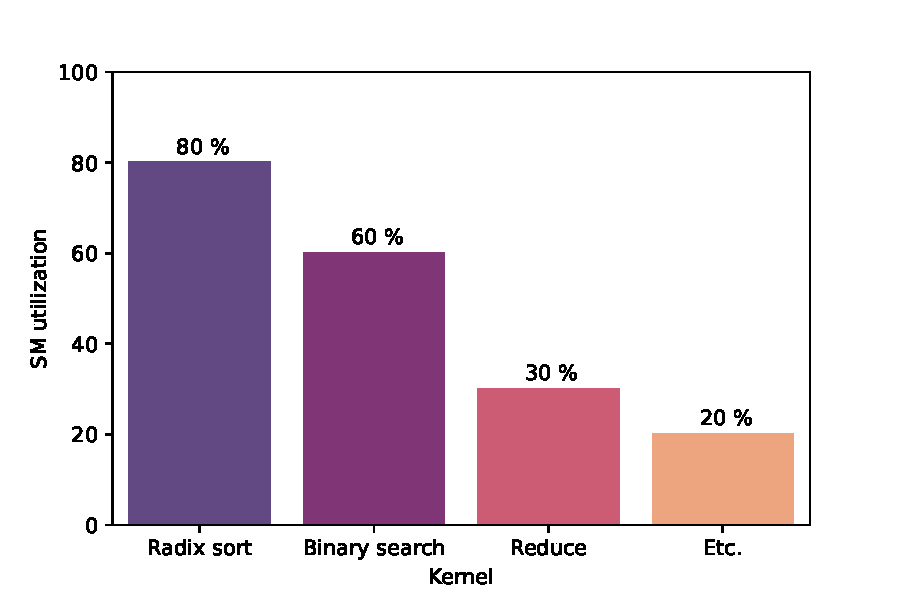
\includegraphics[width=\linewidth]{pictures/fig_2_bar.pdf}
    %       \caption{Производительность процессора}
    %       \label{fig:my_label}
    %   \end{figure}
    %   \end{minipage}
    %   \begin{minipage}{0.45\linewidth}
    %   \begin{figure}
    %       \centering
    %       \includegraphics[width=0.65\linewidth]{pictures/fig2-pie.pdf}
    %       \caption{Время выполнения}
    %       \label{fig:my_label}
    %   \end{figure}
    %   \end{minipage}
    
    \begin{block}{Purpose}
    % Apply distillation to provide optimizations for sparse linear algebra programs eventually compiling them into specialized hardware
    Compile sparse linear algebra programs into specialized hardware with fusion in mind
    \end{block}
    \begin{itemize}
    \vfill
        \item Distillation provides fusion for free for a functional language
        \vfill
        \item Functional language $\to$ specialized hardware? 
        % \vfill
        % \item Specialized hardware mitigates this loss
        % \begin{itemize}
        %     \vfill
        %     \item Extensively used for sparse applications
        %     \vfill
        %     \item More efficient than GPUs/CPUs counterparts
        % \end{itemize}
    \end{itemize}
      
\end{frame}


\begin{frame}[fragile] \frametitle{Hardware synthesis}

    \begin{itemize}
        \item Modern high-level synthesis tools do not handle arbitrary recursion
        \vfill
        \item We utilize FHW --- Haskell to hardware compiler
        \vfill
        \begin{itemize}
            \item Experimental
            \vfill
            \item Arbitrary recursion
            \vfill
            \item Parallel and pipelined dataflow representation
            \vfill
            \begin{itemize}
                \item Easily extensible with, e.g., custom memory
            \end{itemize}
            \vfill
            \item Hardware garbage collection (not present yet)
            \vfill
            \item External Core GHC feature as a frontend
            \begin{itemize}
                \item Removed from GHC > 7.6.3
            \end{itemize}
            \vfill
            \item No external memory support
            \vfill
            \begin{itemize}
                \item Data lives in code 
            \end{itemize}
        \end{itemize}
    \end{itemize}
      
\end{frame}


\begin{frame}[fragile] \frametitle{Data structures}

    \begin{itemize}
        \item Fusion result depends on the underlying data structure
        \vfill
        \item Widely used CSR, COO, etc. do not fit
        \vfill
        \item We use purely functional quad-tree representation
    \end{itemize}
    
\vspace{1cm}

\begin{minted}{Haskell}

  data QTree a = QNone  
               | QVal a 
               | QNode (QTree a) (QTree a)
                       (QTree a) (QTree a) 
  
 \end{minted}

\end{frame}

\begin{frame}[fragile] \frametitle{Plan}

    \begin{itemize}
        \item Get FHW compiler to work
        \vfill
        \item Carry out first experiments
        \vfill
        \item Mitigate GHC 7.6.3 dependency
        \vfill
        \item Add support for external memory
        \vfill
        \item Run full-fledged experiments
    \end{itemize}
      
\end{frame}

\begin{frame}[fragile] \frametitle{Get FHW compiler to work}
  \begin{itemize}
      \item Involved a lot of dataflow and System Verilog debugging
      \vfill
      \item Fixed bugs
      \vfill
      \item Added support for the datatypes of arbitrary size
      \vfill
      \item Automated test workflow
  \end{itemize}
\end{frame}

\begin{frame}[fragile]\frametitle{Compare distilled and non-distilled programs in hardware (small matrices)}

\begin{figure}
    \centering
    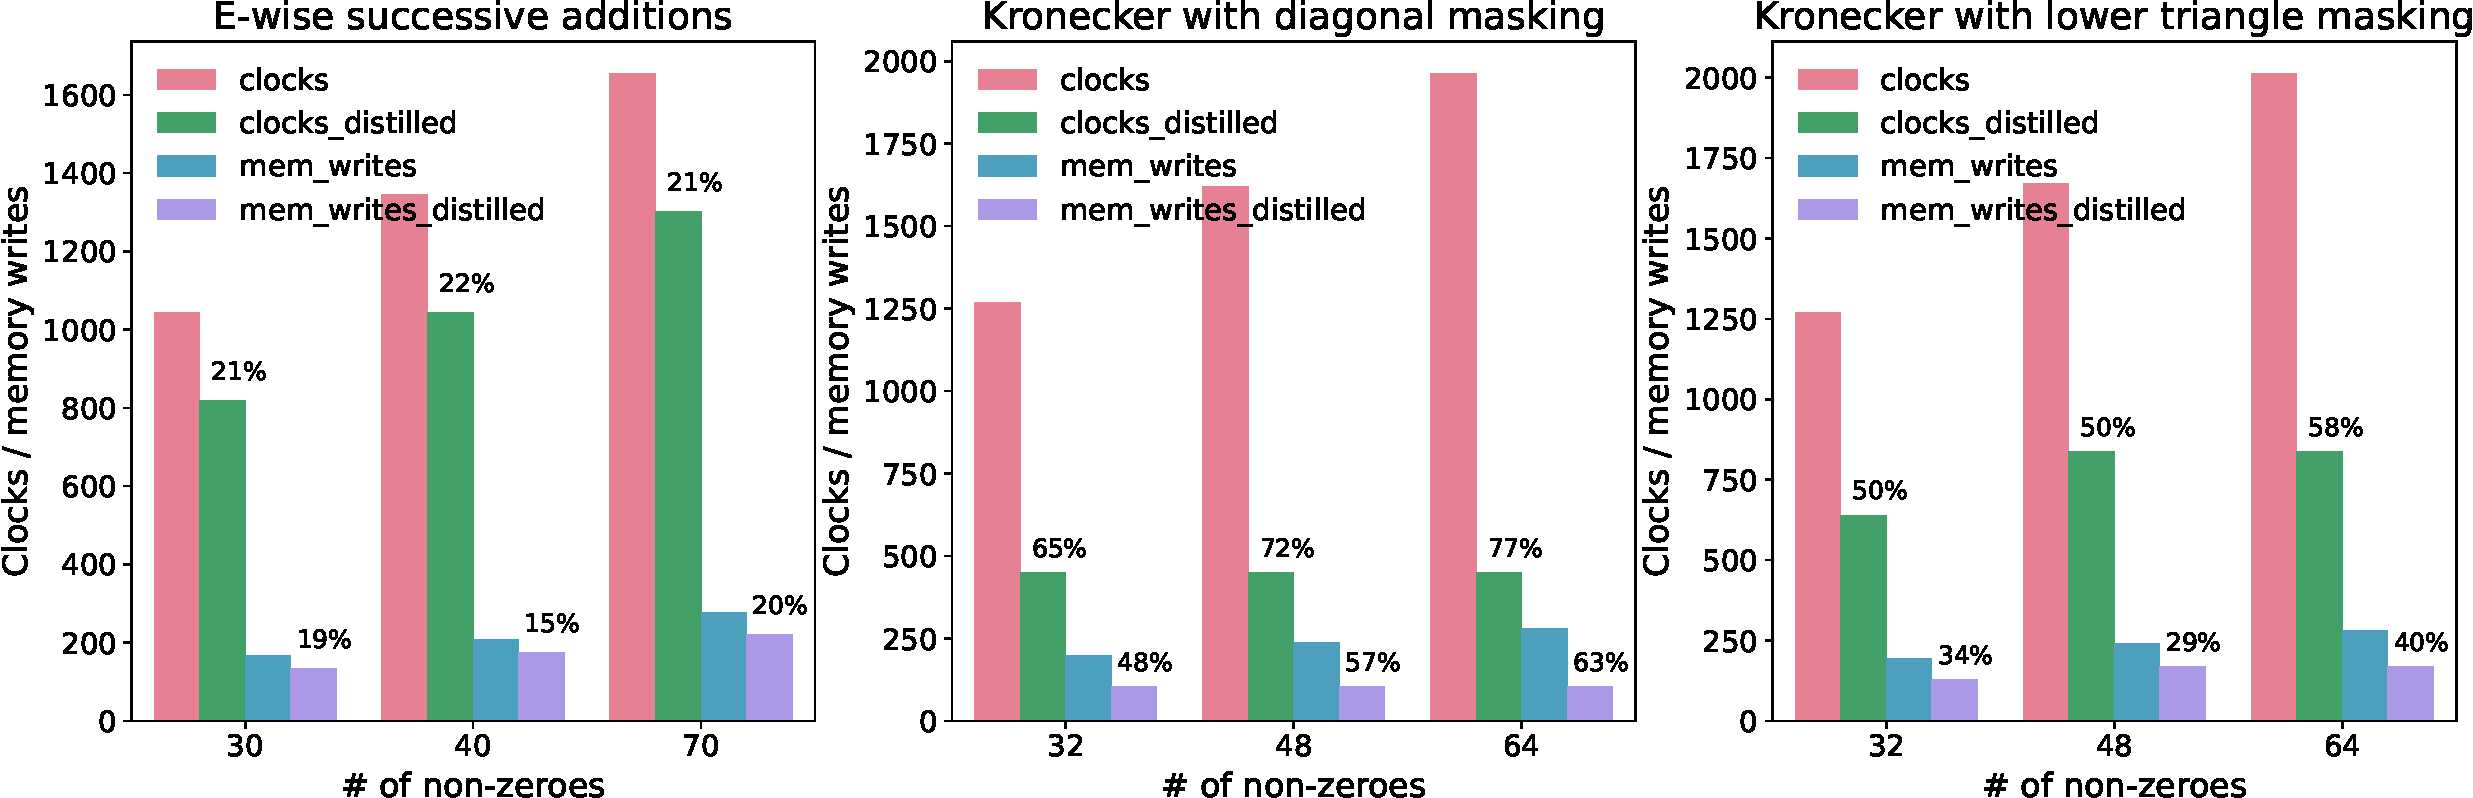
\includegraphics[width=\textwidth]{pictures/HardwareBenchs.pdf}
    % \caption{Experiments for small matrices}
    \label{fig:my_label}
\end{figure}

% \begin{itemize}
%     \vfill
%     \item Compared distilled and non-distilled programs in hardware
% \end{itemize}
    
\end{frame}


\begin{frame}[fragile]\frametitle{Compare distilled and non-distilled programs in hardware (larger matrices)}

\centering
\begin{tabular}{ |l|c|c|c|c|c|c|c|} 
\hline
\rowcolor{LightBlue}
{Function} & {$m_1$} & {$m_2$} & {$m_3$} & {clock ratio} & {time ratio}\\
\hline
\multirow{2}{7em}{E-wise additions} & 64 & 64 & 64 & 0.94 $\pm 0.04$ & 0.94 $\pm 0.04$\\
{} & \rowcolor{LightRed} 128 & 128 & 128 & 0.94 $\pm 0.04$ & 0.95 $\pm 0.04$\\
\hline
\multirow{3}{7em}{Masked addition} & 64 & 64 & 64 & 0.6 $\pm 0.17$ & 0.9 $\pm 0.07$\\
{} & \rowcolor{LightRed} 128 & 128 & 128 & 0.6 $\pm 0.17$ & 0.9 $\pm 0.09$\\
{} & 256 & 256 & 256 & 0.6 $\pm 0.17$ & 0.9 $\pm 0.08$\\
\hline
\multirow{3}{7em}{Masked kron} & \rowcolor{LightRed} 64 & 2 & 128 & 0.16 $\pm 0.03$ & 0.35 $\pm 0.06$\\
{} & 64 & 4 & 256 & 0.27 $\pm 0.03$ & 0.37 $\pm 0.05$\\
{} & \rowcolor{LightRed} 128 & 2 & 256 & 0.19 $\pm 0.01$ & 0.38 $\pm 0.03$\\
\hline
\multirow{3}{7em}{Map addition} &  64 & 64 & 64 & 0.93 $\pm 0.15$ & 0.92 $\pm 0.06$\\
{} & \rowcolor{LightRed} 128 & 128 & 128 & 0.94 $\pm 0.14$ & 0.92 $\pm 0.07$\\
{} &  128 & 2 & 256 & 0.94 $\pm 0.16$ & 0.92 $\pm 0.07$\\
\hline
\end{tabular}


% \begin{itemize}
%     \vfill
%     \item Compared distilled and non-distilled programs in hardware
% \end{itemize}

\end{frame}

\begin{frame}{Move from GHC 7.6.3}
    \begin{itemize}
        \item We use GRIN framework as a middleware between frontend language of the distiller and dataflow backend
        \vfill
        \item It offers whole program optimization
        \vfill
        \item CPS and defunctionalization are more convenient
    \end{itemize}
\end{frame}


\begin{frame}{Results and plans}
    \begin{itemize}
        \item[\faCheck] We have the first evaluation
        \vfill
        \item[\faCheck] Working dataflow backend\footnote{\url{https://github.com/sedwards-lab/fhw}}
        \vfill
        \item[\faCheck] GRIN support for the frontend language\footnote{\url{https://github.com/Tiltedprogrammer/SparseLinAlgHardware}}
        \vfill
        \item[\faCheck] ICFP 2021 SRC poster (and few rejected ones)
        \vfill
        \item[\faGear] GRIN $\to$ dataflow
        \vfill
        \item[\faGear] External memory support
        \vfill
        \item[\faGear] More mature evaluation
        \vfill
        \item[\faGear] GrApl or YArch
    \end{itemize}
\end{frame}


% \begin{frame}[fragile]{Результаты и планы}
%     \begin{itemize}
%         \item[\faCheck] Проведено исследование предметной области
%         \vfill
%         \item[\faCheck] Сформулированы требования к программной и аппаратной частям
%         \vfill
%         \item[\faCheck] Рассмотрены доступные языки в качестве фронтенда (Futhark)
%         \vfill
%         \item[\faCheck] Подано две работы на GrAPL и YArch вокршопы соответственно
%         \vfill
%         \item[\faCheck] Обнаружены и исправлены некоторые из ошибок в FHW
%         \vfill
%         \item Поставить первые эксперименты в симуляции, используя FHW + HOSC
%         \vfill
%         \item Отказаться от GHC и масштабировать решение ...
%     \end{itemize}
% \end{frame}


\end{document}